\documentclass[11pt]{article}

\usepackage[margin=0.9in]{geometry}
\usepackage[T1]{fontenc}
\usepackage{lmodern}
\usepackage{microtype}
\usepackage{amsmath,amssymb}
\usepackage{booktabs}
\usepackage{tabularx}
\usepackage{array}
\usepackage{enumitem}
\usepackage{xcolor}
\usepackage{tikz}
\usetikzlibrary{arrows.meta,positioning,shapes.geometric,calc}
\usepackage{graphicx}
\usepackage[section]{placeins}
\graphicspath{{figures/}}
\usepackage{xurl}
\usepackage[colorlinks=true,linkcolor=blue!50!black,urlcolor=blue!50!black,citecolor=blue!50!black]{hyperref}

\newcolumntype{Y}{>{\raggedright\arraybackslash}X}
\newcolumntype{P}[1]{>{\raggedright\arraybackslash}p{#1}}
\setlist{itemsep=1pt,topsep=3pt}
\emergencystretch=3em
\newcommand{\code}[1]{\texttt{#1}}
\newcommand{\pth}[1]{\nolinkurl{#1}}

% Shared diagram styles: one look for every TikZ figure.
\tikzset{
  box/.style={draw, rounded corners, align=center, font=\small, minimum height=0.8cm, inner sep=4pt},
  good/.style={box, fill=green!15},
  bad/.style={box, fill=red!10},
  plain/.style={box, fill=gray!8},
  arr/.style={-{Latex[length=2.2mm]}, thick},
  fail/.style={-{Latex[length=2.2mm]}, dashed, red!60!black},
  note/.style={font=\footnotesize, align=center},
}

\title{Reinforcement Learning for Lean Proofs\\with a Small Language Model\\[4pt]
\large Midterm report: formulation, experiments, and findings}
\author{Manas Ravulapalli}
\date{13 October 2026}

\begin{document}
\maketitle

\begin{abstract}
This report asks whether reinforcement learning (RL) can teach a small language model, \code{Qwen2.5-0.5B-Instruct}, to write Lean~4 proofs of elementary number theory.
We formulate proof writing as a Markov decision process (MDP) with a reward of 1 only for a complete proof that Lean accepts.
Most experiments failed for one main reason: when the model never succeeds, the RL update is exactly zero.
RL helped only on tasks that the model could already solve some of the time.
We also found ways to obtain the reward without proof skill, and several engineering faults.
\end{abstract}

\noindent\fbox{\parbox{\dimexpr\textwidth-2\fboxsep-2\fboxrule}{
\textbf{Main findings}
\begin{enumerate}[leftmargin=*]
\item RL needs the model to succeed some of the time. With no success, the gradient is zero (Section~\ref{sec:zero}).
\item The first barrier was the Lean language, not the mathematics (Section~\ref{sec:cold}).
\item A reward that does not check correctness can increase while accuracy decreases (Section~\ref{sec:rlpexp}).
\item RL helped twice, both times on tasks that the model could already solve some of the time (Sections~\ref{sec:local} and~\ref{sec:interactive}).
\item A Lean acceptance does not always show skill: the checker had faults, and some statements are trivial (Section~\ref{sec:cheat}).
\item The next run uses a corrected environment, a curriculum ordered by proof structure, and a held-out panel cleaned of tasks that restate training statements (Section~\ref{sec:next}).
\end{enumerate}
}}

%======================================================================
\section{The problem}
\label{sec:problem}

We want a small language model that writes proofs that the proof assistant Lean~4 can check.
The topic is school and early-university number theory: parity, divisibility, gcd and lcm, primes, and congruences.
The midterm goal was a model that produces some complete proofs that Lean accepts.
The goal for the end of the semester is proof strategy on competition-style problems.

\paragraph{Motivation.}
\begin{enumerate}
\item \textbf{Efficiency.} We want the most proofs for a fixed compute budget. We study the \emph{curriculum} (which tasks, in which order) and the \emph{distribution of reward} over proof steps.
\item \textbf{Checked learning.} A model that learns without a checker can learn false statements. Lean should check the model while it learns, not only at the end.
\item \textbf{One model for informal and formal steps.} The model writes a short informal step and then its Lean step. A separate translator would add errors and compute.
\item \textbf{No human graders.} Lean gives an exact reward. This setting is called RL with verifiable rewards (RLVR). The reward is \emph{sparse}: a signal comes only from a complete proof.
\end{enumerate}

\paragraph{What Lean does.}
A Lean theorem has a statement and a proof.
We write the proof as a list of \emph{tactics}.
Each tactic changes the \emph{goals}, the facts that remain to be proved.
When no goals remain, the proof is complete.
Table~\ref{tab:example} shows a small example that we wrote to explain the idea, and Figure~\ref{fig:checker} shows when Lean accepts a proof.

\begin{table}[!htbp]
\centering
\small
\caption{A tactic proof that $a \mid b$ and $b \mid c$ imply $a \mid c$ (here $a \mid b$ means $b = ak$). This example explains the idea; it is not a measured proof.}
\label{tab:example}
\begin{tabularx}{\textwidth}{@{}rP{4.6cm}P{4.3cm}Y@{}}
\toprule
Step & Goal before the step & Tactic (the action) & Effect \\
\midrule
1 & $a \mid c$, given $a \mid b$, $b \mid c$ & \code{obtain $\langle$k, hk$\rangle$ := h1} & Adds $b = a k$ \\
2 & $a \mid c$, given $b = ak$, $b \mid c$ & \code{obtain $\langle$l, hl$\rangle$ := h2} & Adds $c = b l$ \\
3 & $a \mid c$, given $b = ak$, $c = bl$ & \code{exact $\langle$k * l, by rw [hl, hk, Nat.mul\_assoc]$\rangle$} & $c = (ak)l = a(kl)$. No goals remain \\
\bottomrule
\end{tabularx}
\end{table}

\begin{figure}[!htbp]
\centering
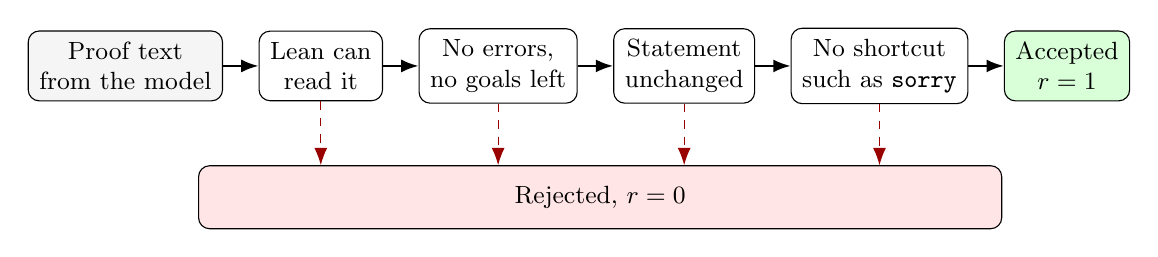
\begin{tikzpicture}[node distance=0.45cm]
\node[plain] (in) {Proof text\\from the model};
\node[box, right=of in] (c1) {Lean can\\read it};
\node[box, right=of c1] (c2) {No errors,\\no goals left};
\node[box, right=of c2] (c3) {Statement\\unchanged};
\node[box, right=of c3] (c4) {No shortcut\\such as \code{sorry}};
\node[good, right=of c4] (ok) {Accepted\\$r = 1$};
\foreach \a/\b in {in/c1, c1/c2, c2/c3, c3/c4, c4/ok} \draw[arr] (\a) -- (\b);
\path (c1.south) -- (c4.south) coordinate[midway] (mid);
\node[bad, minimum width=10.2cm] (no) at ($(mid)+(0,-1.2)$) {Rejected, $r = 0$};
\foreach \n in {c1, c2, c3, c4} \draw[fail] (\n.south) -- (no.north -| \n.south);
\end{tikzpicture}
\caption{When Lean accepts a proof. Every check must pass. One wrong character or one invented lemma name causes a rejection.}
\label{fig:checker}
\end{figure}

\paragraph{Setup.}
Model: \code{Qwen/Qwen2.5-0.5B-Instruct}~\cite{qwen25}, with 494,032,768 parameters.
Checker: Lean \code{v4.10.0-rc1} with one fixed mathlib version.
Compute: one rented NVIDIA L40S GPU, and a shared CPU server.

%======================================================================
\section{Formulation as an MDP}
\label{sec:mdp}

An MDP describes an agent that acts step by step~\cite{suttonbarto}.
At step $t$, the agent observes a state $s_t$, selects an action $a_t$, receives a reward $r_t$, and moves to a state $s_{t+1}$.
Here the agent (the \emph{policy} $\pi_\theta$) is the language model, and the environment is Lean.
We used two formulations, which differ only in the size of one action (Figure~\ref{fig:formab}).

\begin{figure}[!htbp]
\centering
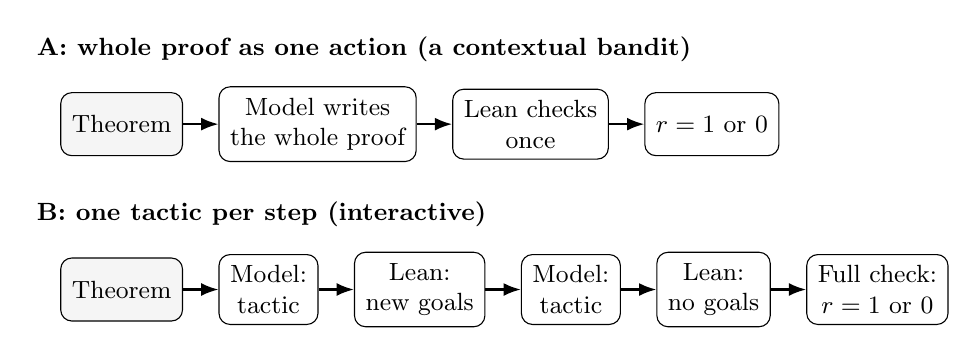
\begin{tikzpicture}[node distance=0.45cm]
\node[font=\small\bfseries, anchor=west] at (-1.2, 0.95) {A: whole proof as one action (a contextual bandit)};
\node[plain] (a0) at (0,0) {Theorem};
\node[box, right=of a0] (a1) {Model writes\\the whole proof};
\node[box, right=of a1] (a2) {Lean checks\\once};
\node[box, right=of a2] (a3) {$r = 1$ or $0$};
\foreach \x/\y in {a0/a1, a1/a2, a2/a3} \draw[arr] (\x) -- (\y);
\node[font=\small\bfseries, anchor=west] at (-1.2, -1.15) {B: one tactic per step (interactive)};
\node[plain] (b0) at (0,-2.1) {Theorem};
\node[box, right=of b0] (b1) {Model:\\tactic};
\node[box, right=of b1] (b2) {Lean:\\new goals};
\node[box, right=of b2] (b3) {Model:\\tactic};
\node[box, right=of b3] (b4) {Lean:\\no goals};
\node[box, right=of b4] (b5) {Full check:\\$r = 1$ or $0$};
\foreach \x/\y in {b0/b1, b1/b2, b2/b3, b3/b4, b4/b5} \draw[arr] (\x) -- (\y);
\end{tikzpicture}
\caption{The two formulations. In A, the model receives no feedback while it writes (Experiments 4 to 6, 20 to 22). In B, Lean runs each tactic first (Experiments 19 and 23).}
\label{fig:formab}
\end{figure}

Table~\ref{tab:mdp} defines Formulation B, and Figure~\ref{fig:mdpgraph} shows it as a graph.

\begin{table}[!htbp]
\centering
\small
\caption{The interactive MDP (environment version 1).}
\label{tab:mdp}
\begin{tabularx}{\textwidth}{@{}P{2.6cm}Y@{}}
\toprule
Part & Definition \\
\midrule
State $s_t$ & The current Lean goals. At $t = 0$, the theorem. In an \emph{assisted} task, part of a known proof is applied first \\
Action $a_t$ & A short tactic block (at most 64 tokens in the main run) \\
Transition & Lean runs the block. If it succeeds, the new goals are $s_{t+1}$ \\
End of episode & No goals remain (then Lean checks the full proof), Lean reports an error, or the step budget is used (4 actions) \\
Reward & 1 at the end if Lean accepts the full proof, otherwise 0 \\
Discount & $\gamma = 1$ \\
\bottomrule
\end{tabularx}
\end{table}

\begin{figure}[!htbp]
\centering
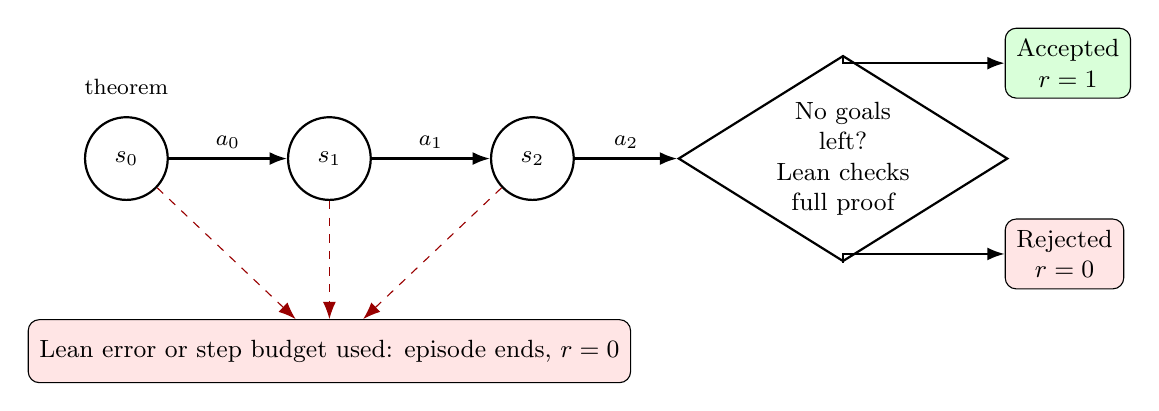
\begin{tikzpicture}[st/.style={circle, draw, thick, minimum size=1.05cm, font=\small}]
\node[st] (s0) {$s_0$};
\node[st, right=1.5cm of s0] (s1) {$s_1$};
\node[st, right=1.5cm of s1] (s2) {$s_2$};
\node[diamond, draw, thick, aspect=1.6, align=center, font=\small, inner sep=1pt, right=1.3cm of s2] (chk) {No goals\\left?\\Lean checks\\full proof};
\node[good, above right=0.1cm and 1.0cm of chk] (win) {Accepted\\$r = 1$};
\node[bad, below right=0.1cm and 1.0cm of chk] (lose) {Rejected\\$r = 0$};
\node[bad, below=1.5cm of s1] (err) {Lean error or step budget used: episode ends, $r = 0$};
\draw[arr] (s0) -- node[above, note] {$a_0$} (s1);
\draw[arr] (s1) -- node[above, note] {$a_1$} (s2);
\draw[arr] (s2) -- node[above, note] {$a_2$} (chk);
\draw[arr] (chk) |- (win);
\draw[arr] (chk) |- (lose);
\foreach \n in {s0, s1, s2} \draw[fail] (\n) -- (err);
\node[above=0.15cm of s0, note] {theorem};
\end{tikzpicture}
\caption{Formulation B for the proof of Table~\ref{tab:example}. Solid arrows: the tactic succeeds. Dashed arrows: an error ends the episode with reward 0.}
\label{fig:mdpgraph}
\end{figure}

Version 1 has three defects.
The model does not see the remaining steps, the theorem, or the proof so far.
With a step limit that the model cannot see, the process is not exactly Markov.
One error ends the episode.
Section~\ref{sec:next} corrects these defects.

\subsection{Learning algorithm}
We maximize the expected return $J(\theta) = \mathbb{E}_{\tau \sim \pi_\theta}\big[\sum_t \gamma^t r_t\big]$.
The only reward is at the end, so the return of an episode $\tau$ is $R(\tau) \in \{0, 1\}$.
For one theorem, we sample $G$ episodes and use the REINFORCE estimator~\cite{williams1992}
\begin{equation}
\nabla_\theta J(\theta) \approx \frac{1}{G}\sum_{i=1}^{G} A_i \, \nabla_\theta \log \pi_\theta(\tau_i).
\label{eq:pg}
\end{equation}
The \emph{advantage} $A_i$ compares attempt $i$ with the other attempts.
The interactive runs use the leave-one-out baseline (RLOO)~\cite{ahmadian2024}, and the whole-proof runs use GRPO~\cite{shao2024,trl}:
\begin{equation}
A_i^{\text{RLOO}} = R_i - \frac{1}{G-1}\sum_{j \neq i} R_j, \qquad
A_i^{\text{GRPO}} = \frac{R_i - \bar R}{s_R + \varepsilon},
\label{eq:rloo}
\end{equation}
where $\bar R$ and $s_R$ are the mean and standard deviation of the $G$ rewards.

\subsection{Main consequence: no success, no learning}
\label{sec:zero}
If all $G$ attempts fail, every $R_i = 0$, so every $A_i = 0$, and the update in Equation~\eqref{eq:pg} is exactly zero.
The same is true when all attempts succeed.
The model learns only from \emph{mixed groups}, which contain at least one success and one failure (Figure~\ref{fig:groups}).

\begin{figure}[!htbp]
\centering
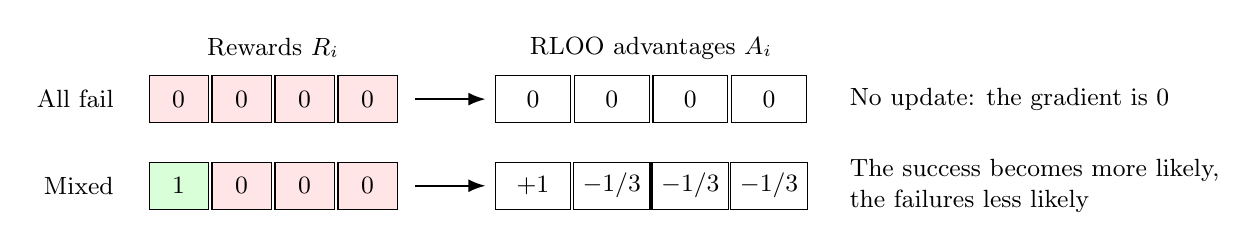
\begin{tikzpicture}[
  cell/.style={draw, minimum width=0.75cm, minimum height=0.6cm, font=\small},
  lab/.style={font=\small, anchor=east, align=right}]
\node[lab] at (-0.3, 0) {All fail};
\foreach \i/\r in {0/0,1/0,2/0,3/0} \node[cell, fill=red!10] at (0.8*\i+0.4, 0) {$\r$};
\draw[arr] (3.4, 0) -- (4.3, 0);
\foreach \i/\a in {0/0,1/0,2/0,3/0} \node[cell, minimum width=0.95cm] at (1.0*\i+4.9, 0) {$\a$};
\node[font=\small, anchor=west, align=left] at (8.8, 0) {No update: the gradient is 0};
\node[lab] at (-0.3, -1.1) {Mixed};
\foreach \i/\r/\c in {0/1/green!15,1/0/red!10,2/0/red!10,3/0/red!10} \node[cell, fill=\c] at (0.8*\i+0.4, -1.1) {$\r$};
\draw[arr] (3.4, -1.1) -- (4.3, -1.1);
\foreach \i/\a in {0/{+1},1/{-1/3},2/{-1/3},3/{-1/3}} \node[cell, minimum width=0.95cm] at (1.0*\i+4.9, -1.1) {$\a$};
\node[font=\small, anchor=west, align=left] at (8.8, -1.1) {The success becomes more likely,\\the failures less likely};
\node[font=\small] at (1.6, 0.65) {Rewards $R_i$};
\node[font=\small] at (6.4, 0.65) {RLOO advantages $A_i$};
\end{tikzpicture}
\caption{A group needs both a success and a failure ($G = 4$).}
\label{fig:groups}
\end{figure}

If the model succeeds with probability $p$ per attempt, a group of $G$ independent attempts is mixed with probability
\begin{equation}
P_{\text{mix}}(p, G) = 1 - p^{G} - (1-p)^{G}.
\label{eq:pmix}
\end{equation}
Figure~\ref{fig:pmix} shows that this probability is small when $p$ is small.
This equation explains most of our failures.

\begin{figure}[!htbp]
\centering
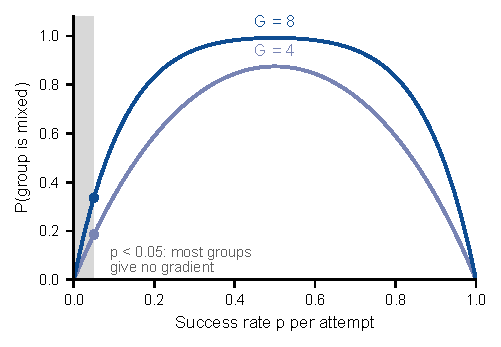
\includegraphics[width=0.45\textwidth]{pmix}
\caption{Probability that a group is mixed (Equation~\ref{eq:pmix}). At $p = 0.05$ it is 0.185 for $G = 4$ and 0.337 for $G = 8$.}
\label{fig:pmix}
\end{figure}

\subsection{A second reward: RLP}
\label{sec:rlp}
Some experiments used the RLP reward~\cite{rlp} instead of Lean.
For a question $x$, reasoning $c$, and known answer $y$, the reward is $\log p_\theta(y \mid x, c) - \log p_{\bar\theta}(y \mid x)$, where $p_{\bar\theta}$ is a slowly updated copy of the model.
The reward is high when the reasoning makes the correct answer more probable.
It does not check whether the reasoning is correct (Figure~\ref{fig:rewards}).
We call it a \emph{heuristic} reward.

\begin{figure}[!htbp]
\centering
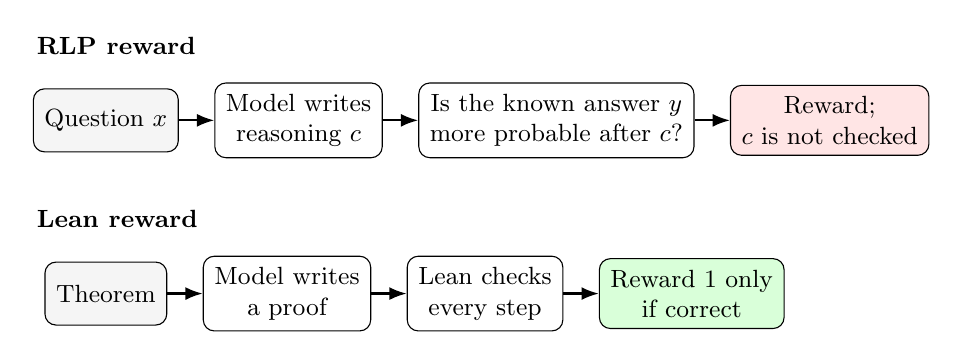
\begin{tikzpicture}[node distance=0.45cm]
\node[font=\small\bfseries, anchor=west] at (-1.0, 0.95) {RLP reward};
\node[plain] (x) at (0,0) {Question $x$};
\node[box, right=of x] (c) {Model writes\\reasoning $c$};
\node[box, right=of c] (q) {Is the known answer $y$\\more probable after $c$?};
\node[bad, right=of q] (r) {Reward;\\$c$ is not checked};
\foreach \a/\b in {x/c, c/q, q/r} \draw[arr] (\a) -- (\b);
\node[font=\small\bfseries, anchor=west] at (-1.0, -1.25) {Lean reward};
\node[plain] (t) at (0,-2.2) {Theorem};
\node[box, right=of t] (p) {Model writes\\a proof};
\node[box, right=of p] (l) {Lean checks\\every step};
\node[good, right=of l] (r2) {Reward 1 only\\if correct};
\foreach \a/\b in {t/p, p/l, l/r2} \draw[arr] (\a) -- (\b);
\end{tikzpicture}
\caption{The two rewards. RLP rewards reasoning that makes a known answer more probable, correct or not. Lean rewards only a correct proof.}
\label{fig:rewards}
\end{figure}

\paragraph{Measures.}
\emph{Accepted attempts} counts sampled proofs that Lean accepts, for example 26/48.
\emph{Theorem coverage} counts theorems with at least one accepted attempt.
One standard tactic proves 28 of the 420 validation statements without a model, so the main validation set is the other 392 (\emph{non-trivial}) statements.

%======================================================================
\section{Data, training stages, and curricula}
\label{sec:data}

\begin{table}[!htbp]
\centering
\small
\caption{Data sources and their use.}
\label{tab:data}
\begin{tabularx}{\textwidth}{@{}P{3.4cm}YP{3.4cm}@{}}
\toprule
Source & Content & Use \\
\midrule
LeanDojo Benchmark 4~\cite{leandojo} & Theorems and tactic proofs from mathlib; number-theory subset of 706 training, 17 validation, 15 test theorems & Supervised training; short proofs for interactive RL \\
Lean Workbook~\cite{leanworkbook} & Competition-style problems as Lean statements & Pool of 4,306 number-theory statements that Lean checks \\
Number-theory SFT set & 5,812 examples: Lean-accepted proofs, mathlib syntax examples, proof variants & Second supervised stage \\
Hand-written Lean tasks & Logic, arithmetic, divisibility, induction & Experiments 5, 6; DEV of Experiment 19 \\
Hand-written arithmetic tasks & 448 questions on gcd, inverses, primes, congruences & RLP (Experiment 9) \\
Open textbook (Judson) & Chapters of \emph{Abstract Algebra: Theory and Applications} & RLP (Experiment 7) \\
Curriculum templates & 192 training tasks in 5 stages and 152 held-out tasks, all checked by Lean & Final run (Section~\ref{sec:next}) \\
\bottomrule
\end{tabularx}
\end{table}

Table~\ref{tab:data} lists the data.
Figure~\ref{fig:splits} shows how we keep test data out of training.
Renamed copies of one problem always go to the same split, and we never train on the DEV set.

\begin{figure}[!htbp]
\centering
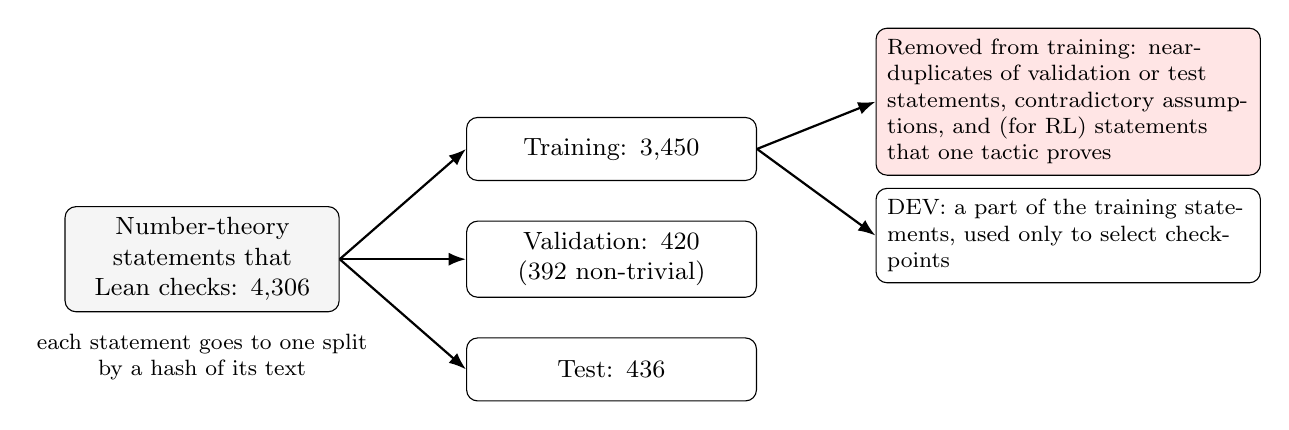
\begin{tikzpicture}
\node[plain, text width=3.2cm] (pool) at (0, 0) {Number-theory statements that Lean checks: 4,306};
\node[note, below=0.15cm of pool] {each statement goes to one split\\by a hash of its text};
\node[box, text width=3.4cm] (tr) at (5.2, 1.4) {Training: 3,450};
\node[box, text width=3.4cm] (val) at (5.2, 0) {Validation: 420\\(392 non-trivial)};
\node[box, text width=3.4cm] (te) at (5.2, -1.4) {Test: 436};
\foreach \n in {tr, val, te} \draw[arr] (pool.east) -- (\n.west);
\node[bad, text width=4.6cm, align=left, font=\footnotesize] (rm) at (11.0, 2.0) {Removed from training: near-duplicates of validation or test statements, contradictory assumptions, and (for RL) statements that one tactic proves};
\node[box, text width=4.6cm, align=left, font=\footnotesize] (dev) at (11.0, 0.3) {DEV: a part of the training statements, used only to select checkpoints};
\draw[arr] (tr.east) -- (rm.west);
\draw[arr] (tr.east) -- (dev.west);
\end{tikzpicture}
\caption{Data splits. Two statements are near-duplicates when their token sets overlap by at least 85\%.}
\label{fig:splits}
\end{figure}

\paragraph{Training stages.}
All models come from one chain of checkpoints (Figure~\ref{fig:pipeline}).
SFT v2 is one pass over Lean proofs from the LeanDojo training files (4,526 steps of 64 examples), without any file that contains a validation or test theorem.
Common SFT is a second supervised stage on the number-theory SFT set.
Supervised fine-tuning (SFT) copies existing proofs.
RL learns from the model's own attempts, so some attempts must succeed.

\begin{figure}[!htbp]
\centering
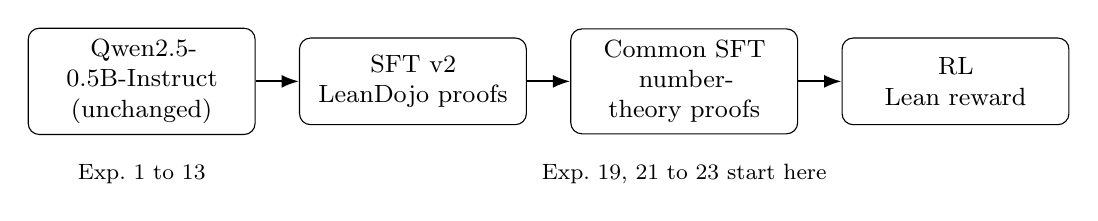
\begin{tikzpicture}[st/.style={box, minimum height=1.1cm, text width=2.6cm}]
\node[st] (a) {Qwen2.5-0.5B-Instruct\\(unchanged)};
\node[st, right=0.55cm of a] (b) {SFT v2\\LeanDojo proofs};
\node[st, right=0.55cm of b] (c) {Common SFT\\number-theory proofs};
\node[st, right=0.55cm of c] (d) {RL\\Lean reward};
\draw[arr] (a) -- (b);
\draw[arr] (b) -- (c);
\draw[arr] (c) -- (d);
\node[below=0.25cm of a, note] {Exp.\ 1 to 13};
\node[below=0.25cm of c, note] {Exp.\ 19, 21 to 23 start here};
\end{tikzpicture}
\caption{The training chain.}
\label{fig:pipeline}
\end{figure}

\paragraph{Curricula.}
RL needs tasks that the model can solve some of the time.
A \emph{curriculum} starts with easier versions of a task.
We made tasks easier in three ways: we supplied knowledge in the prompt, we supplied part of the proof (a \emph{reverse curriculum}~\cite{r3}, Figure~\ref{fig:reverse}), or we asked for one step instead of a whole proof.
Most known proofs are short: 85\% of the linear tactic proofs in our LeanDojo pool have one or two tactics, and only 24 have five or more.
Therefore a reverse curriculum on these proofs has few levels.
To test whether \emph{order} matters, an \emph{ordered} arm and a \emph{shuffled} arm receive the same tasks the same number of times.
Table~\ref{tab:curricula} lists the curriculum of each experiment.

\begin{figure}[!htbp]
\centering
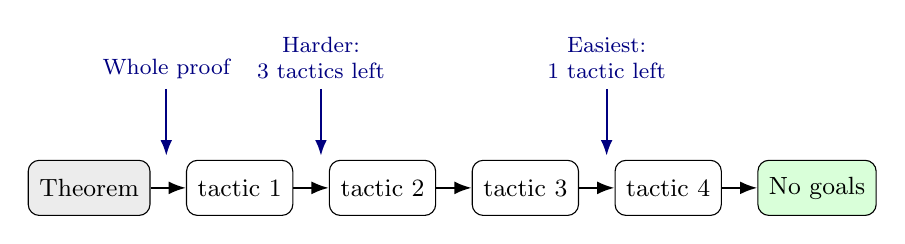
\begin{tikzpicture}[
  tac/.style={box, minimum width=1.35cm, minimum height=0.7cm, fill=#1},
  tac/.default=white,
  st/.style={-{Latex[length=2mm]}, thick, blue!50!black}]
\node[tac=gray!15] (thm) {Theorem};
\node[tac, right=0.45cm of thm] (t1) {tactic 1};
\node[tac, right=0.45cm of t1] (t2) {tactic 2};
\node[tac, right=0.45cm of t2] (t3) {tactic 3};
\node[tac, right=0.45cm of t3] (t4) {tactic 4};
\node[tac=green!15, right=0.45cm of t4] (qed) {No goals};
\draw[arr] (thm) -- (t1); \draw[arr] (t1) -- (t2); \draw[arr] (t2) -- (t3); \draw[arr] (t3) -- (t4); \draw[arr] (t4) -- (qed);
\draw[st] ($(t4.north west)+(-0.1,0.9)$) node[above, note] {Easiest:\\1 tactic left} -- ($(t4.north west)+(-0.1,0.05)$);
\draw[st] ($(t2.north west)+(-0.1,0.9)$) node[above, note] {Harder:\\3 tactics left} -- ($(t2.north west)+(-0.1,0.05)$);
\draw[st] ($(t1.north west)+(-0.25,0.9)$) node[above, note] {Whole proof} -- ($(t1.north west)+(-0.25,0.05)$);
\end{tikzpicture}
\caption{A reverse curriculum on one known proof. Each blue arrow is a start point; the earlier tactics are given. Training moves the start point toward the theorem.}
\label{fig:reverse}
\end{figure}

\begin{table}[!htbp]
\centering
\small
\caption{Curricula by experiment.}
\label{tab:curricula}
\begin{tabularx}{\textwidth}{@{}P{1.0cm}P{4.2cm}YP{2.3cm}@{}}
\toprule
Exp. & Tasks & Order and support & Comparison \\
\midrule
4 & LeanDojo number-theory theorems & Grouped by topic & Random order \\
5 & Hand-written Lean tasks & Logic, arithmetic, divisibility, induction; support decreases & Random order \\
6 & Theorems with part of the proof given & Missing expression, then tactic, then body & Random order \\
9 & 448 arithmetic tasks & Prerequisites first, with replay & None \\
13 & 72 tasks in 5 versions & Support decreases from full information to none & Shuffled order \\
20 & Number-theory proofs & Short proof endings, longer endings, whole proofs & SFT parent \\
19 & 3 practice proof endings & Fixed mixture & SFT parent \\
23 & 22 Lean Workbook theorems & Structure, lemma use, combined steps, whole proof & Shuffled order \\
Final & S0 to S4 templates & Identity, one lemma, two steps, chain of subgoals, 3 to 6 steps & Shuffled; adaptive \\
\bottomrule
\end{tabularx}
\end{table}

%======================================================================
\section{Experiments}
\label{sec:experiments}

Figure~\ref{fig:story} shows all experiments in order, with the lesson that led to each next experiment.
A cause is \emph{tested} when an experiment could have shown it to be false; otherwise it is a \emph{candidate}.

\begin{figure}[!htbp]
\centering
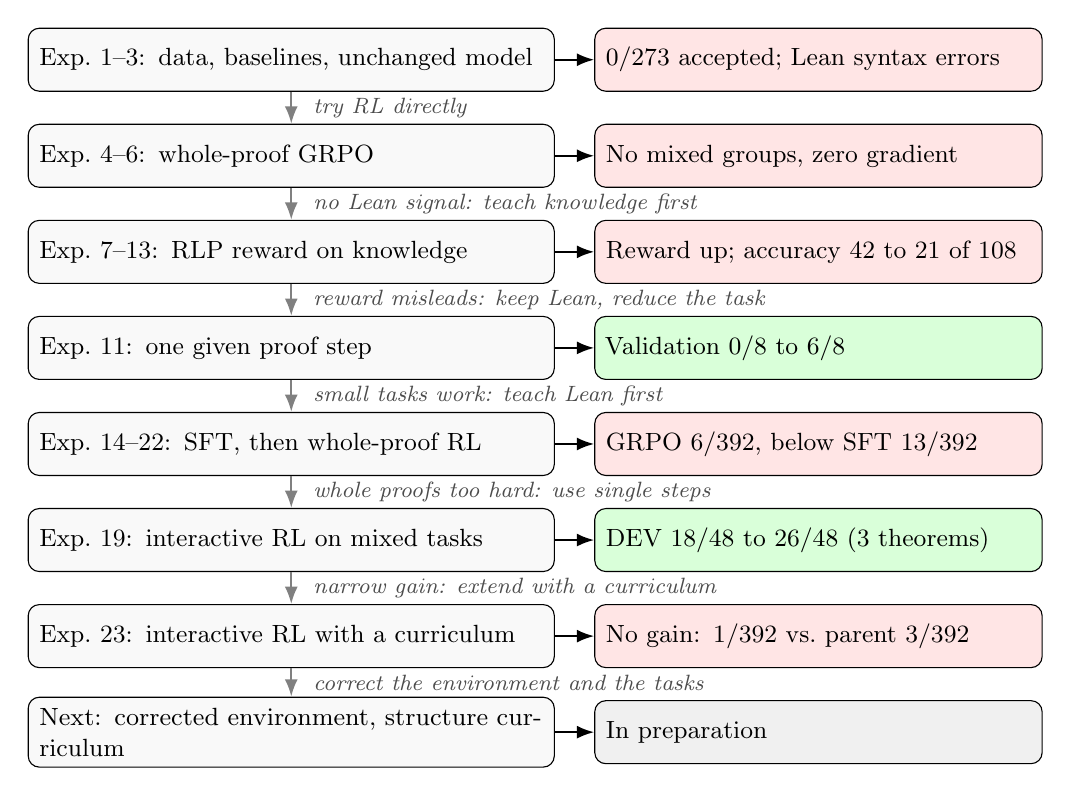
\begin{tikzpicture}[
  exp/.style={box, text width=6.4cm, align=left, fill=gray!5},
  res/.style={box, text width=5.4cm, align=left, fill=#1},
  why/.style={font=\footnotesize\itshape, anchor=west, text=black!70}]
\def\gap{1.22}
\foreach \y/\e/\r/\c in {
  0/{Exp.~1--3: data, baselines, unchanged model}/{0/273 accepted; Lean syntax errors}/red!10,
  1/{Exp.~4--6: whole-proof GRPO}/{No mixed groups, zero gradient}/red!10,
  2/{Exp.~7--13: RLP reward on knowledge}/{Reward up; accuracy 42 to 21 of 108}/red!10,
  3/{Exp.~11: one given proof step}/{Validation 0/8 to 6/8}/green!15,
  4/{Exp.~14--22: SFT, then whole-proof RL}/{GRPO 6/392, below SFT 13/392}/red!10,
  5/{Exp.~19: interactive RL on mixed tasks}/{DEV 18/48 to 26/48 (3 theorems)}/green!15,
  6/{Exp.~23: interactive RL with a curriculum}/{No gain: 1/392 vs.\ parent 3/392}/red!10,
  7/{Next: corrected environment, structure curriculum}/{In preparation}/gray!12}
{
  \node[exp] (e\y) at (0, -\gap*\y) {\e};
  \node[res=\c, right=0.5cm of e\y] (r\y) {\r};
  \draw[arr] (e\y) -- (r\y);
}
\foreach \a/\b/\w in {0/1/{try RL directly}, 1/2/{no Lean signal: teach knowledge first}, 2/3/{reward misleads: keep Lean, reduce the task}, 3/4/{small tasks work: teach Lean first}, 4/5/{whole proofs too hard: use single steps}, 5/6/{narrow gain: extend with a curriculum}, 6/7/{correct the environment and the tasks}}
  \draw[arr, gray] (e\a.south) -- node[pos=0.5, xshift=0.15cm, why] {\w} (e\b.north);
\end{tikzpicture}
\caption{The sequence of experiments. Red: failure. Green: RL gain. Grey: in preparation.}
\label{fig:story}
\end{figure}

%----------------------------------------------------------------------
\subsection{Data, baseline, and the unchanged model (Experiments 1 to 3)}
\label{sec:cold}
Experiment~1 selected a number-theory subset of LeanDojo.
Its authors report that the random split overestimates performance~\cite{leandojo}, so we later built stricter splits (Figure~\ref{fig:splits}).
Experiment~2 tested the base model on school mathematics: 9 of 24 GSM8K and 3 of 20 MATH number-theory problems.
A small fine-tune lowered the held-out loss, but the scores became 8 of 24 and 3 of 20.
A lower loss did not mean better answers.

Experiment~3 asked the unchanged model to prove 21 statements.
Lean accepted 0 of 63 local attempts and 0 of 273 GPU attempts.
Figure~\ref{fig:exp3} shows that no attempt reached the mathematics.
A pattern match found old Lean~3 syntax in 33 of the 63 attempts.
In 34 of the 63, the model wrote a new theorem when we asked only for a proof.
The first barrier is the language (\emph{tested}: the classification reads Lean's error messages).

\begin{figure}[!htbp]
\centering
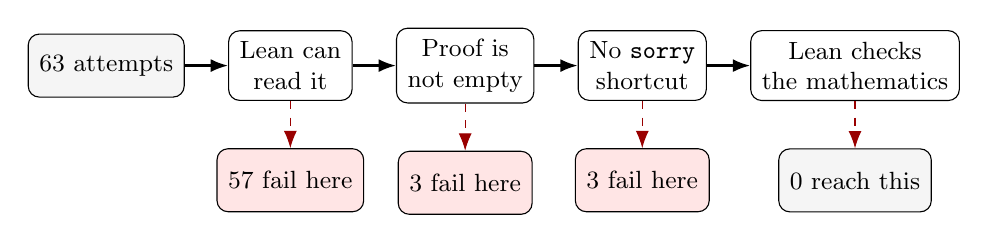
\begin{tikzpicture}[node distance=0.55cm]
\node[plain] (all) {63 attempts};
\node[box, right=of all] (k1) {Lean can\\read it};
\node[box, right=of k1] (k2) {Proof is\\not empty};
\node[box, right=of k2] (k3) {No \code{sorry}\\shortcut};
\node[box, right=of k3] (k4) {Lean checks\\the mathematics};
\foreach \a/\b in {all/k1, k1/k2, k2/k3, k3/k4} \draw[arr] (\a) -- (\b);
\node[bad, below=0.6cm of k1] (f1) {57 fail here};
\node[bad, below=0.6cm of k2] (f2) {3 fail here};
\node[bad, below=0.6cm of k3] (f3) {3 fail here};
\node[plain, below=0.6cm of k4] (f4) {0 reach this};
\foreach \a/\b in {k1/f1, k2/f2, k3/f3, k4/f4} \draw[fail] (\a) -- (\b);
\end{tikzpicture}
\caption{Where the 63 attempts of Experiment 3 failed.}
\label{fig:exp3}
\end{figure}

%----------------------------------------------------------------------
\subsection{Whole-proof RL from the unchanged model (Experiments 4 to 6)}
\label{sec:terminal}
We ran GRPO in Formulation A with $G = 4$.
In Experiment~4, Lean accepted no proof, no group was mixed, and the gradient was zero for all 32 steps.
Validation stayed at 0 of 8 theorems.
In Experiment~5, easier hand-written tasks gave 0 of 256 accepted proofs, so we did not train.
In Experiment~6, with one expression missing from a given proof, 2 of 64 attempts passed, but only one theorem gave mixed groups, and held-out attempts stayed at 0 of 16.

\emph{Why it failed} (\emph{tested}): every group had reward 0, so every update was 0 (Section~\ref{sec:zero}).
Therefore Experiment~4 gives no information about curriculum order.

%----------------------------------------------------------------------
\subsection{RL with a reward that does not check correctness (Experiments 7 to 10, 12, 13)}
\label{sec:rlpexp}
Lean gave no signal, so we tried to teach knowledge first with the RLP reward.
\begin{itemize}
\item Experiment 7 (textbook text): held-out accuracy was 11/48 before and after.
\item Experiment 8: only 8,557,971 of 494,032,768 weights had changed, because low-precision (BF16) rounding discards small updates. With full precision, accuracy stayed at 11/48.
\item Experiment 9 (448 arithmetic tasks): the reward increased, but held-out accuracy decreased from 42/108 to 21/108 (Figure~\ref{fig:rlpdiv}). Answers without a readable number increased from 17 to 69, and answers at the length limit from 15 to 36.
\item Experiment 10: an early checkpoint improved at recognizing concepts (7 to 14 of 32), not at using them. Two AI graders disagreed on 44 of 321 answers.
\item Experiment 12: all 612 numeric answers in the data were correct, but 160 of 448 rules omitted a condition (for example, $\gcd(a, n) = 1$ for a modular inverse). A constant answer solved every proof-by-contradiction item.
\item Experiment 13 (decreasing support): 0 of 18 answers were fully correct at all five checkpoints.
\end{itemize}

\begin{figure}[!htbp]
\centering
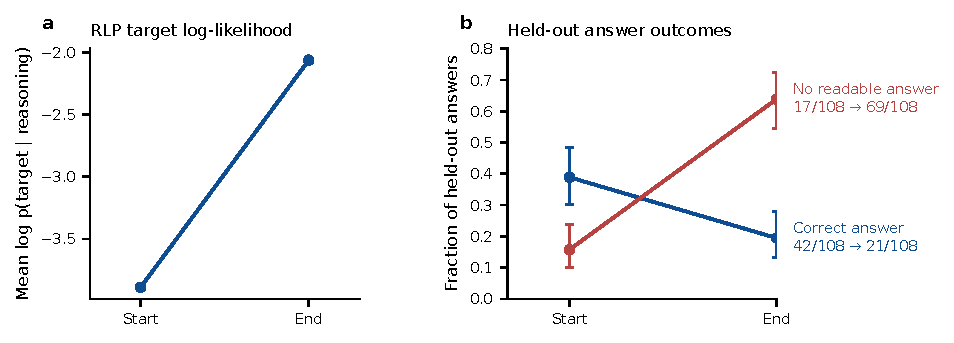
\includegraphics[width=0.75\textwidth]{rlp_divergence}
\caption{Experiment 9. (a)~The quantity that the RLP reward pays for increased. (b)~Held-out answers, $n = 108$. Error bars: 95\% Wilson score intervals.}
\label{fig:rlpdiv}
\end{figure}

\emph{Why it failed}: the reward pays for reasoning that makes the answer more probable, not for correct reasoning.
This is \emph{reward hacking}.
In Experiment~9, 17 incorrect answers received a positive advantage.
A deliberately false line of reasoning increased the reward in both inspected examples.
A \emph{candidate} reason for the accuracy decrease is that training supplied the start of the answer format, but the test did not.

%----------------------------------------------------------------------
\subsection{A smaller task (Experiment 11)}
\label{sec:local}
We reduced the task to one proof step with the mathematics supplied (Figure~\ref{fig:exp11}), and ran GRPO with $G = 8$.
Validation accuracy increased from 0/8 to 6/8, and held-out accuracy from 0/4 to 2/4.
It worked because some groups were mixed.
The sets are small, and Lean checked only the expression: only 2 of 8 explanations had no mathematical error.

\begin{figure}[!htbp]
\centering
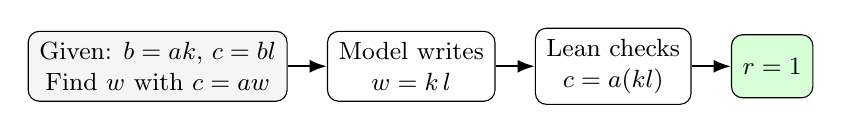
\begin{tikzpicture}[node distance=0.5cm]
\node[plain] (g) {Given: $b = ak$, $c = bl$\\Find $w$ with $c = a w$};
\node[box, right=of g] (m) {Model writes\\$w = k\,l$};
\node[box, right=of m] (l) {Lean checks\\$c = a(kl)$};
\node[good, right=of l] (r) {$r = 1$};
\draw[arr] (g) -- (m); \draw[arr] (m) -- (l); \draw[arr] (l) -- (r);
\end{tikzpicture}
\caption{The one-step task of Experiment 11. Lean checks the expression, not the explanation.}
\label{fig:exp11}
\end{figure}

%----------------------------------------------------------------------
\subsection{Supervised training, then whole-proof RL (Experiments 14 to 22)}
\label{sec:sftrl}
After SFT v2, the model solved 0 of the 392 non-trivial validation statements (2 of all 420).
On 200 training statements it proved 0 in 1,600 attempts.
The most frequent first errors were an invented lemma name (582), a failed rewrite (329), and the length limit (253).
The barrier moved from syntax to library knowledge.

Experiment~20 added a common SFT stage, then alternated SFT with whole-proof GRPO in one branch and with RLP in another (Figure~\ref{fig:interleaved}).
Common SFT increased the count from 0 to 13.
The GRPO branch ended at 6, below its parent, and the RLP branch at 15.
The GRPO model wrote the single tactic \code{simp\_all} in 1,637 of 3,360 samples; the parent did so in 62.

\begin{figure}[!htbp]
\centering
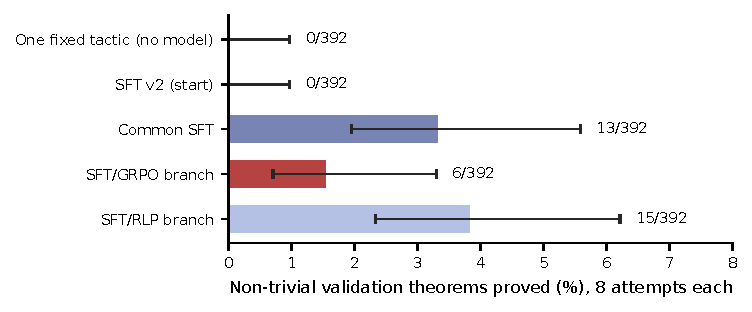
\includegraphics[width=0.65\textwidth]{interleaved}
\caption{Experiment 20: non-trivial validation statements with an accepted proof in 8 attempts, $n = 392$. Error bars: 95\% Wilson score intervals.}
\label{fig:interleaved}
\end{figure}

Experiment~21 used rejection-sampling fine-tuning (RFT: train on sampled proofs that Lean accepts~\cite{deepseekprover15}), then GRPO.
On DEV (64 attempts per model), no model had an accepted proof.
The first errors of the final model were proof construction (43), unknown names or types (17), syntax (3), and timeout (1).
A parser fault rejected every action in a code block, so its step-by-step pilot made no update.
Experiment~22 prepared PPO, but the GPU run failed before RL started.

\emph{Why it failed} (\emph{candidates}): the low success rate gives few mixed groups; the GRPO model concentrated on \code{simp\_all}, which closes only easy goals.
The branches also had extra SFT stages and different data, so the comparison does not isolate RL.

%----------------------------------------------------------------------
\subsection{Step-by-step RL: the clear gain (Experiment 19)}
\label{sec:interactive}
We used Formulation B from common SFT, with REINFORCE, RLOO, $G = 4$, and at most 4 actions.
We trained only on three practice tasks that the model solved some of the time.
The success rule, fixed before the run, required more accepted DEV attempts than the parent over two seeds and no lost DEV theorem.
The rule selected the RL model (Figure~\ref{fig:mixed}).
It proved 7 of 32 original theorems without help (parent: 4 of 32), and all 7 proofs passed a new Lean check.
An earlier run of this type lost one DEV theorem, so the rule kept its parent.
Not every theorem improved: \code{Nat.not\_even\_one} decreased from 4/4 to 2/4.

\begin{figure}[!htbp]
\centering
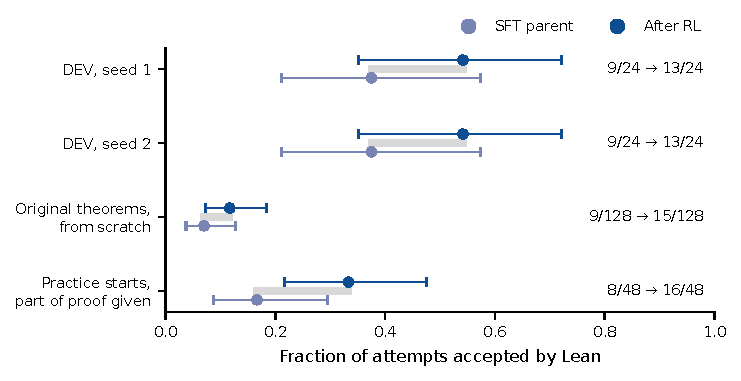
\includegraphics[width=0.7\textwidth]{mixed_gain}
\caption{Experiment 19: SFT parent and RL model on the same tasks and seeds. Error bars: 95\% Wilson score intervals, which treat correlated attempts as independent and so understate the uncertainty.}
\label{fig:mixed}
\end{figure}

\emph{Limits}: DEV has only 3 theorems, there is one training seed, and the 32 original theorems are from the training domain.
RL made the model more reliable on proofs that it could already find; it did not show that RL teaches new proofs.

%----------------------------------------------------------------------
\subsection{Step-by-step RL with a curriculum (Experiment 23)}
\label{sec:curriculum}
On 22 broader theorems, a short warm-start first increased whole-proof success on 16 training tasks from 0 to 13.
Then an \emph{ordered} arm (answer given, one lemma, combined steps, whole proof) and a \emph{shuffled} arm trained on the same tasks.
Neither arm improved on the parent.
On broader DEV, all three models had 0 of 64.
On easy retention, the parent had 24/48, ordered 20/48, and shuffled 21/48.
On non-trivial validation, the parent proved 3 of 392 and ordered RL 1 of 392; one of the parent's accepted statements has the empty set as an answer.
The ordered model made more valid first moves than the parent (88 against 40), but it completed no proof in its first move (Figure~\ref{fig:curriculum}).

\begin{figure}[!htbp]
\centering
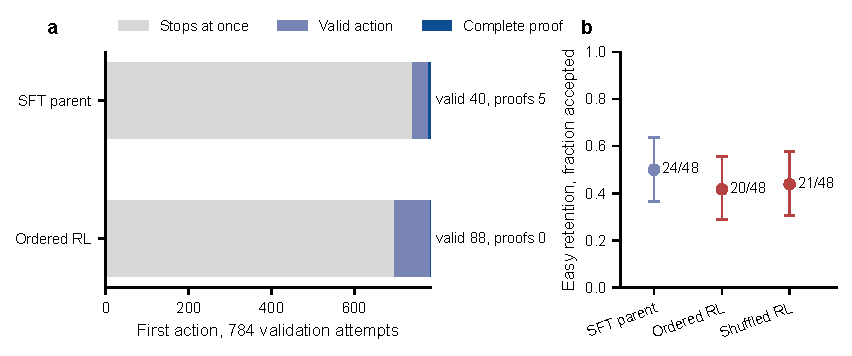
\includegraphics[width=0.8\textwidth]{curriculum_outcome}
\caption{Experiment 23. (a)~First action on the same 784 validation attempts. (b)~Easy retention, $n = 48$. Error bars: 95\% Wilson score intervals.}
\label{fig:curriculum}
\end{figure}

\emph{Why it failed} (four \emph{candidates}, not yet tested):
\begin{enumerate}
\item A valid step is not progress. The model learned valid steps, not complete proofs.
\item The curriculum had gaps: the lemma stage covered 9 of 22 theorems, the combined stage 11 of 22, and early tasks contained the answer.
\item For one Lean error type, the interface lost the message and gave reward 0, while ordinary errors received a penalty. A failure with a lost message therefore scored better (186 actions).
\item The environment did not show the theorem or the remaining steps, and one error ended the episode.
\end{enumerate}
One common explanation is not supported: most repeated-state failures occurred without \code{simp\_all}.

%======================================================================
\section{Ways to obtain the reward without proof skill}
\label{sec:cheat}
We searched for every way to obtain the Lean reward without real proof skill and found six types (Figure~\ref{fig:cheat}).

\begin{figure}[!htbp]
\centering
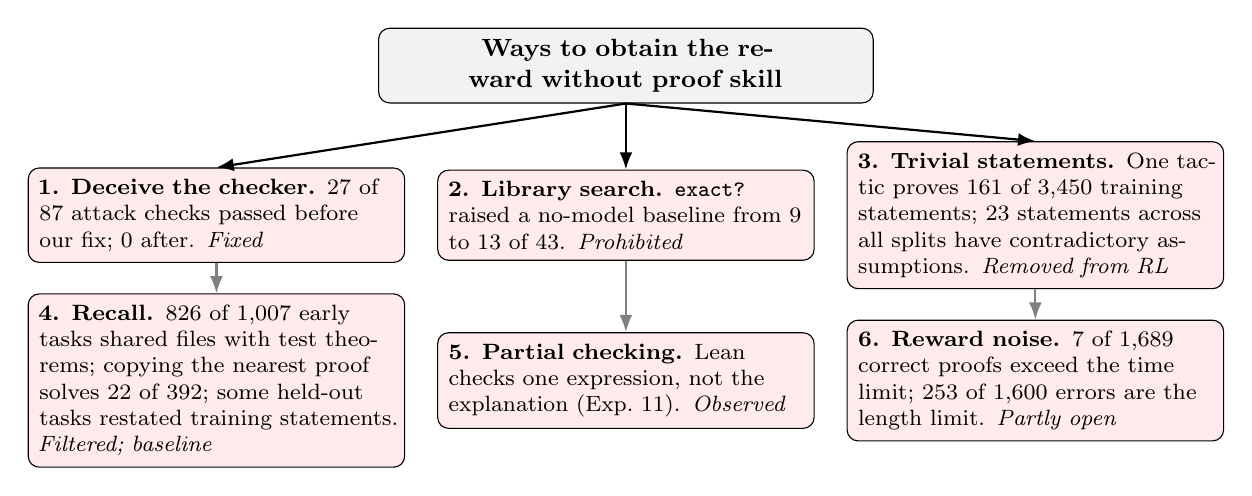
\begin{tikzpicture}[leaf/.style={box, text width=4.5cm, align=left, font=\footnotesize, fill=#1}, leaf/.default=red!8]
\node[box, text width=6cm, fill=gray!10] (root) at (0, 0) {\textbf{Ways to obtain the reward without proof skill}};
\node[leaf] (a) at (-5.2, -1.9) {\textbf{1. Deceive the checker.} 27 of 87 attack checks passed before our fix; 0 after. \emph{Fixed}};
\node[leaf] (b) at (0, -1.9) {\textbf{2. Library search.} \code{exact?} raised a no-model baseline from 9 to 13 of 43. \emph{Prohibited}};
\node[leaf] (c) at (5.2, -1.9) {\textbf{3. Trivial statements.} One tactic proves 161 of 3,450 training statements; 23 statements across all splits have contradictory assumptions. \emph{Removed from RL}};
\node[leaf] (d) at (-5.2, -4.0) {\textbf{4. Recall.} 826 of 1,007 early tasks shared files with test theorems; copying the nearest proof solves 22 of 392; some held-out tasks restated training statements. \emph{Filtered; baseline}};
\node[leaf] (e) at (0, -4.0) {\textbf{5. Partial checking.} Lean checks one expression, not the explanation (Exp.~11). \emph{Observed}};
\node[leaf] (f) at (5.2, -4.0) {\textbf{6. Reward noise.} 7 of 1,689 correct proofs exceed the time limit; 253 of 1,600 errors are the length limit. \emph{Partly open}};
\foreach \n in {a, b, c} \draw[arr] (root.south) -- (\n.north);
\foreach \n/\m in {d/a, e/b, f/c} \draw[arr, gray] (\m.south) -- (\n.north);
\end{tikzpicture}
\caption{Six types of reward without real proof skill, with measurements and status.}
\label{fig:cheat}
\end{figure}

The checker attacks included false ``no axioms'' messages, a replaced axiom report, and a command after the proof.
A scan of 10,869 accepted proofs found no attack in real runs.
Some statements are also formalized incorrectly; for example, a divisibility statement about $(5 + \sqrt{35})^{2n-1}$ is about real numbers, where it is trivially true.
Before we report an RL gain, we therefore separate trivial, contradictory, near-duplicate, and new statements, and report the new statements.

%======================================================================
\section{Engineering faults}
\label{sec:bugs}

\begin{table}[!htbp]
\centering
\small
\caption{Engineering faults that we found.}
\label{tab:bugs}
\begin{tabularx}{\textwidth}{@{}P{3.8cm}YP{2.7cm}@{}}
\toprule
Fault & Effect & Status \\
\midrule
BF16 optimizer state & Small updates rounded away & Fixed (full precision) \\
Checker attacks & 27 of 87 attack checks accepted & Fixed (0 of 87) \\
Batch checking & One broken proof caused the rejection of the next proof; 15 of 40 correct proofs rejected in one test & Fixed \\
Action parser & Every action in a code block rejected before Lean & Fixed \\
Lost Lean error messages & One error type gave reward 0 instead of a penalty (186 actions) & Patch not yet verified \\
Proof export & Indentation of multi-line proofs changed, so exports failed & Fixed \\
Full-file compilation & DEV files exceeded the memory limit without a proof & Open \\
Prohibited-word filter & A string trick hid a prohibited command, and Lean accepted it & Fixed (version 2.2) \\
Run failures & Full disk at checkpoint save; missing PPO method; launch-script name conflict; wrong prompt-length count & Fixed \\
\bottomrule
\end{tabularx}
\end{table}

Some failures were engineering faults, not scientific results (Table~\ref{tab:bugs}).

%======================================================================
\section{Next steps}
\label{sec:next}

\paragraph{Corrected environment.}
Version 2.1 of the environment corrects the defects of version 1 (Figure~\ref{fig:v2}).
The model sees the theorem, the accepted steps, the current goals, the last Lean message, the tactics that already failed, and the remaining steps.
An action contains up to four tactics, and Lean keeps all tactics before the first error, as in DeepSeek-Prover-V1.5~\cite{deepseekprover15}.
The reward is 1 for a proof and 0 otherwise, with $\gamma = 0.95$, so shorter proofs receive more reward.
Version 2.2 corrected further faults.
Integration tests with real Lean passed: 8 of 8 for version 2.1, and 86 of 86 for the version 2.2 trainer.

\begin{figure}[!htbp]
\centering
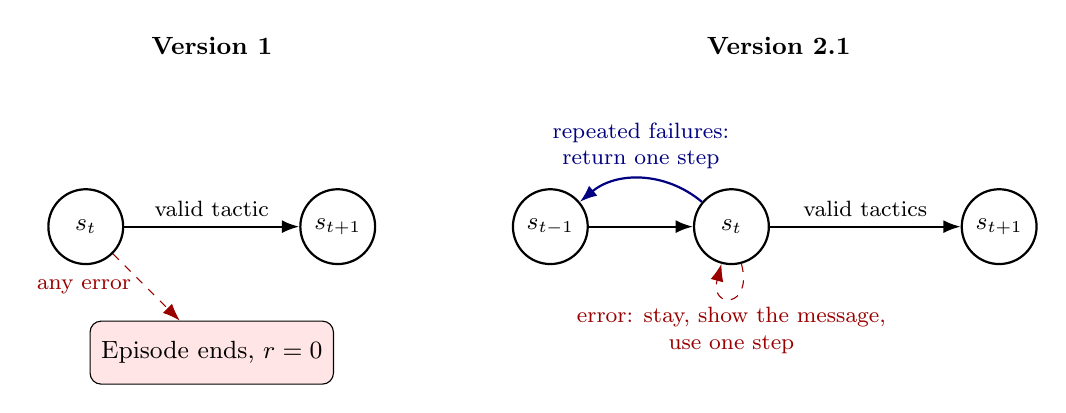
\begin{tikzpicture}[st/.style={circle, draw, thick, minimum size=0.95cm, font=\small}]
\node[font=\small\bfseries] at (1.6, 2.3) {Version 1};
\node[st] (a) at (0, 0) {$s_t$};
\node[st] (b) at (3.2, 0) {$s_{t+1}$};
\node[bad] (e) at (1.6, -1.6) {Episode ends, $r = 0$};
\draw[arr] (a) -- node[above, note] {valid tactic} (b);
\draw[fail] (a) -- node[left, note, xshift=-2pt] {any error} (e);
\begin{scope}[xshift=7.2cm]
\node[font=\small\bfseries] at (1.6, 2.3) {Version 2.1};
\node[st] (p) at (-1.3, 0) {$s_{t-1}$};
\node[st] (c) at (1.0, 0) {$s_t$};
\node[st] (d) at (4.4, 0) {$s_{t+1}$};
\draw[arr] (p) -- (c);
\draw[arr] (c) -- node[above, note] {valid tactics} (d);
\draw[fail] (c) edge[loop below, looseness=6] node[below, note] {error: stay, show the message,\\use one step} (c);
\draw[arr, blue!50!black] (c) to[bend right=40] node[above, note] {repeated failures:\\return one step} (p);
\end{scope}
\end{tikzpicture}
\caption{Treatment of a failed action in version 1 and version 2.1.}
\label{fig:v2}
\end{figure}

\paragraph{Curriculum ordered by proof structure.}
The final curriculum has five stages, ordered by the type of reasoning that a proof needs (Figure~\ref{fig:stairs}).
All tasks come from templates in families of 8, and Lean accepts the reference proof of every task.
A family that one fixed tactic mostly solves (4 or more of 8) moves to S0.
We defined this relabel rule after we saw the first probe results, so it was not chosen blind.
Within the training set, exact duplicates were removed, which leaves 192 training tasks.

\begin{figure}[!htbp]
\centering
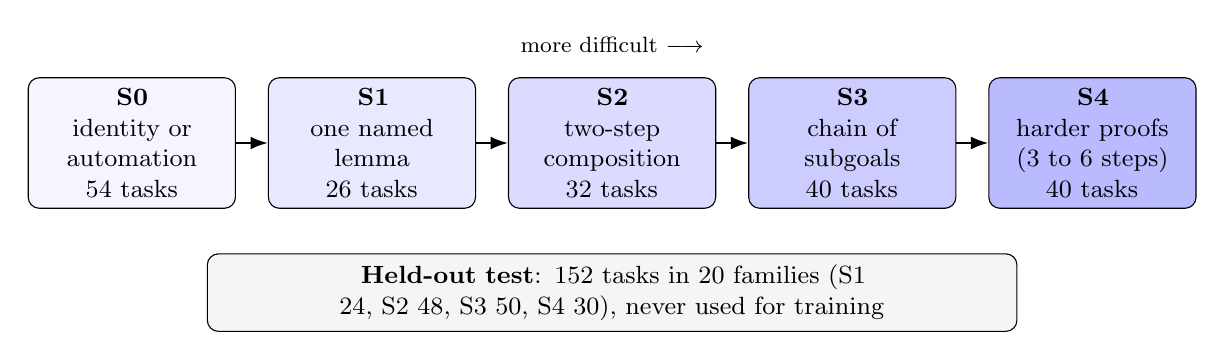
\begin{tikzpicture}[stp/.style={box, text width=2.35cm, minimum height=1.3cm}]
\node[stp, fill=blue!4]  (s0) at (0, 0)    {\textbf{S0}\\identity or\\automation\\54 tasks};
\node[stp, fill=blue!9]  (s1) at (3.05, 0) {\textbf{S1}\\one named\\lemma\\26 tasks};
\node[stp, fill=blue!14] (s2) at (6.1, 0)  {\textbf{S2}\\two-step\\composition\\32 tasks};
\node[stp, fill=blue!20] (s3) at (9.15, 0) {\textbf{S3}\\chain of\\subgoals\\40 tasks};
\node[stp, fill=blue!27] (s4) at (12.2, 0) {\textbf{S4}\\harder proofs\\(3 to 6 steps)\\40 tasks};
\foreach \a/\b in {s0/s1, s1/s2, s2/s3, s3/s4} \draw[arr] (\a) -- (\b);
\node[note] at (6.1, 1.25) {more difficult $\longrightarrow$};
\node[plain, text width=10cm] (ho) at (6.1, -1.9) {\textbf{Held-out test}: 152 tasks in 20 families (S1 24, S2 48, S3 50, S4 30), never used for training};
\end{tikzpicture}
\caption{The final structure curriculum: 192 training tasks and 152 held-out tasks. Training excludes 670 names: every held-out, evaluation, reserve, demo, and DEV name.}
\label{fig:stairs}
\end{figure}

\paragraph{Cleaning the held-out set.}
A semantic check compared held-out tasks with the statements behind the SFT data.
In the first panel, it found 26 held-out--training pairs with the same content and 3 near-transfers; for example, \code{ho\_coprimechain\_01} restates \code{lean\_workbook\_22701}.
We removed 35 tasks, which left 61 clean tasks.
A second set of new families went through the same check, which removed 7 contaminated held-out families and 2 training families.
We then dropped the 5 remaining held-out tasks rated ``related''.
The final held-out set has 152 tasks: the 61 original clean tasks and 91 new ones.
On the 61 original clean tasks, the SFT parent (environment version 1) solved 6, with 8 of 488 attempts accepted.

\paragraph{Can RL start on these stages?}
Before training, we ran the SFT parent 8 times on each S0 to S2 task of the first template set, with the version~1 prompt (Figure~\ref{fig:probe}).
With the relabelled stages, S0 had 187 of 448 attempts accepted (44 of 56 tasks mixed), S1 26 of 256 (14 of 32 mixed), and S2 10 of 256 (8 of 32 mixed).
Every stage has mixed groups, so RL has a signal, but the signal is weak in S2.
Under the original labels, one family that \code{omega} solves alone gave 32 of the 42 S2 successes, and the two real two-step families gave 8 of 64 and 0 of 64.
With the version 2.1 prompt, 186 of 386 first actions of the parent failed on format.
In 145 of these 186, the code block had a label other than \code{lean}, for example \code{liquorice}; no run has tested whether the label causes the failure.
Therefore a short warm-start in the new format comes before RL.
Its data has 1,969 training rows on 468 theorems, each traced again through the version 2.1 environment.

\begin{figure}[!htbp]
\centering
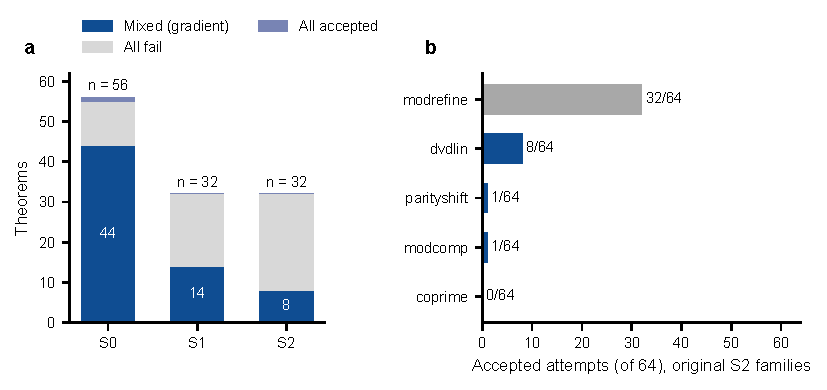
\includegraphics[width=0.8\textwidth]{stage_probe}
\caption{Readiness test of the SFT parent on the first template set, version~1 prompt, 8 attempts per task, one seed. (a)~Tasks per relabelled stage by outcome. (b)~Accepted attempts per family of the original S2 stage, $n = 64$; grey: the family that \code{omega} solves alone, later moved to S0.}
\label{fig:probe}
\end{figure}

\paragraph{The frozen plan for the final run.}
We recorded the protocol before the launch; no result of this run exists yet.
The run tests two claims: RL improves the model over its warm-start W on held-out tasks, and a curriculum makes RL more efficient (Figure~\ref{fig:design}).

\begin{figure}[!htbp]
\centering
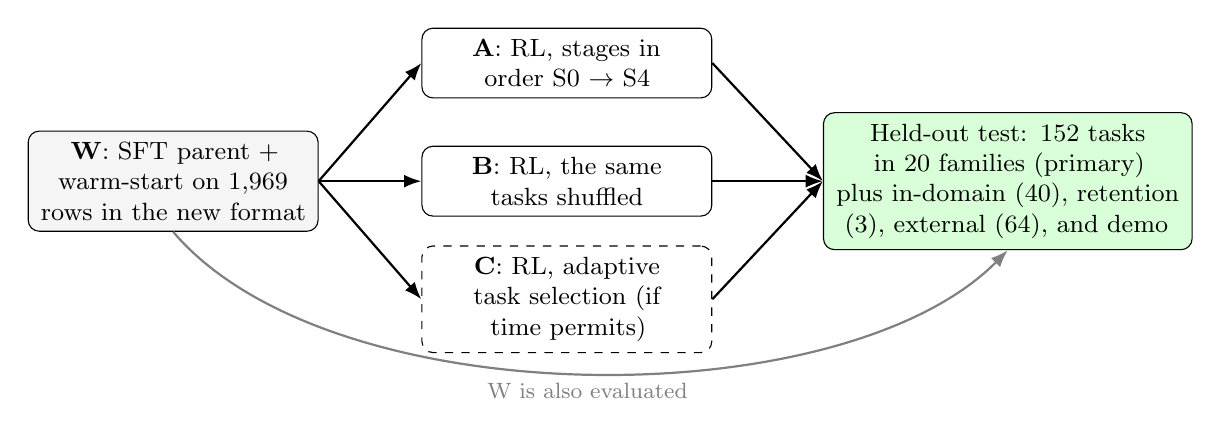
\begin{tikzpicture}[node distance=0.5cm]
\node[plain, text width=3.4cm] (w) at (0, 0) {\textbf{W}: SFT parent + warm-start on 1,969 rows in the new format};
\node[box, text width=3.4cm] (a) at (5.0, 1.5) {\textbf{A}: RL, stages in order S0 $\to$ S4};
\node[box, text width=3.4cm] (b) at (5.0, 0) {\textbf{B}: RL, the same tasks shuffled};
\node[box, text width=3.4cm, dashed] (c) at (5.0, -1.5) {\textbf{C}: RL, adaptive task selection (if time permits)};
\foreach \n in {a, b, c} \draw[arr] (w.east) -- (\n.west);
\node[good, text width=4.4cm] (ev) at (10.6, 0) {Held-out test: 152 tasks in 20 families (primary)\\plus in-domain (40), retention (3), external (64), and demo};
\foreach \n in {a, b, c} \draw[arr] (\n.east) -- (ev.west);
\draw[arr, gray] (w.south) .. controls (2, -3.0) and (8.5, -3.0) .. node[below, note] {W is also evaluated} (ev.south);
\end{tikzpicture}
\caption{The frozen comparison. A and B against W test whether RL helps. A against B tests whether order helps. C tests whether tasks near a 50\% success rate give more mixed groups for the same compute.}
\label{fig:design}
\end{figure}

\begin{itemize}
\item \textbf{Settings.} Environment version 2.2, $\gamma = 0.95$, $G = 8$, at most 6 actions, REINFORCE with the leave-one-out baseline on discounted returns, learning rate $10^{-6}$, seed 20261013 for every arm, at most 150 groups per arm.
\item \textbf{Admission.} W samples each training task 8 times. A task enters training only if 1 to 6 of the 8 attempts succeed, so every admitted task can give mixed groups. A stage with too few admitted tasks is dropped from both arms.
\item \textbf{Primary measure.} The mean fraction of the 8 attempts that Lean accepts, per held-out task. The primary test permutes whole families, because tasks in one family are correlated; Holm correction controls the two comparisons of each claim.
\item \textbf{Efficiency.} For each arm, the gain in solved tasks over W per million generated tokens, together with Lean calls, updates, and the share of mixed groups.
\item \textbf{Validity gates.} A against B counts as confirmatory only if both arms complete the same number of groups, with updates within 10\% and censored groups within 2. The efficiency claim also needs generated tokens within 10\%. If training success does not increase during RL, a null result is uninformative. No checkpoint, setting, or task is chosen from evaluation results.
\item \textbf{Sample size.} In simulation, the McNemar test gave a false-positive rate of up to 0.14 against the intended 0.05; the family test stays at 0.05 or less. With the final 152 tasks, the family test detects 8 to 19 percentage points in the fraction of tasks solved, and 11 to 15 points at a baseline like the parent's. These values come from an assumed model, not from data.
\item \textbf{Compute.} One L4 GPU for 12 hours, with a reservation of USD 37.01 and one attempt. A CPU fallback runs as a labelled deviation if the attempt fails.
\item \textbf{Demo.} \code{demo\_coprime} and one held-out task per level (a common divisor divides the gcd; odd $m$ and $n$ give an even $mn + 1$; $ab$ or $a + b$ is even), run on A if A solves at least as many held-out tasks as W, otherwise on W. Six earlier demo problems matched statements in the training or SFT data and were withdrawn.
\end{itemize}

%======================================================================
\section{Limitations}
\begin{itemize}
\item The evaluation sets are small (3 DEV theorems in Experiment~19; 4 to 8 items in Experiment~11), and every run used one seed.
\item Several sets were reused across experiments, so they now act as development sets.
\item We do not know how much Lean or mathlib the model saw in pretraining.
\item AI reviewers graded the natural-language answers in Experiments 9, 10, 11, and 13.
\item The sample-size values come from simulations with assumed parameters.
\item The numbers come from recorded run outputs; we did not repeat experiments for this report.
\end{itemize}

\paragraph{Sources.}
Each experiment has a record in \pth{docs/EXPERIMENTS.md}.
The earlier detailed report (Git commit \code{e3b7747}) contains every count of Experiments 1 to 13 and the full checker audit.
The reward exploits are in \pth{docs/REWARD_HACKING.md}.
The script \pth{scripts/report/make_report_figures.py} draws the data figures and names the record of each number.

\begin{thebibliography}{99}
\bibitem{qwen25} Qwen Team. Qwen2.5 technical report. \url{https://arxiv.org/abs/2412.15115}.
\bibitem{leandojo} K.~Yang et al. LeanDojo: Theorem proving with retrieval-augmented language models. \url{https://arxiv.org/abs/2306.15626}.
\bibitem{suttonbarto} R.~S.~Sutton and A.~G.~Barto. \emph{Reinforcement Learning: An Introduction}, 2nd edition. MIT Press, 2018.
\bibitem{williams1992} R.~J.~Williams. Simple statistical gradient-following algorithms for connectionist reinforcement learning. \emph{Machine Learning}, 8:229--256, 1992.
\bibitem{ahmadian2024} A.~Ahmadian, C.~Cremer, M.~Gall\'e, et al. Back to basics: Revisiting REINFORCE style optimization for learning from human feedback in LLMs. \url{https://arxiv.org/abs/2402.14740}.
\bibitem{shao2024} Z.~Shao, P.~Wang, Q.~Zhu, et al. DeepSeekMath: Pushing the limits of mathematical reasoning in open language models. \url{https://arxiv.org/abs/2402.03300}.
\bibitem{trl} Hugging Face. TRL v0.24.0 GRPO trainer documentation. \url{https://huggingface.co/docs/trl/v0.24.0/en/grpo_trainer}.
\bibitem{rlp} A.~Hatamizadeh, S.~N.~Akter, S.~Prabhumoye, J.~Kautz, et al. RLP: Reinforcement as a pretraining objective. \url{https://arxiv.org/abs/2510.01265}.
\bibitem{leanworkbook} H.~Ying, Z.~Wu, Y.~Geng, et al. Lean Workbook: A large-scale Lean problem set formalized from natural language math problems. \url{https://arxiv.org/abs/2406.03847}.
\bibitem{r3} Training large language models for reasoning through reverse curriculum reinforcement learning. \url{https://arxiv.org/abs/2402.05808}.
\bibitem{deepseekprover15} H.~Xin et al. DeepSeek-Prover-V1.5: Harnessing proof assistant feedback for reinforcement learning and Monte-Carlo tree search. \url{https://arxiv.org/abs/2408.08152}.
\end{thebibliography}

\end{document}
